\subsection{Reference-Calibrated Comparison With Cited Study-Aligned Methods}
\label{subsec:study_aligned_numerical}

The works in Table~\ref{tab:recent_comparison} use different data sets,
insurance lines, prediction targets and privacy mechanisms, and several do not
simulate an endogenous competitive health-insurance market. Their published
scores therefore cannot be combined into a valid numerical leaderboard. We
instead implement a study-aligned version of each relevant capability inside
the same FL-IMDR market. These rows are capability-matched comparators, not
claims of exact cross-data reproduction.

The \emph{Dong--Quan AutoML-aligned} method performs held-out selection of the
feature family and regularization strength before applying frozen personalized
risk pricing, following the automated insurance-model-selection objective in
\cite{DongQuan2025}. The \emph{Richman et al. credibility-aligned} method uses
sample-size-dependent weighting between each insurer's observed experience and
a portfolio prior, reflecting the credibility mechanism in
\cite{Richman2025}. The \emph{Piontkowski small-portfolio-aligned} method uses
stronger reference-portfolio shrinkage when few accepted members are
available, following the small health-insurance portfolio motivation in
\cite{Piontkowski2025}. The \emph{Xin et al. fairness-aligned} comparator
suppresses direct age and health terms and shrinks personalized risk loads
toward the portfolio mean. This is a fairness-oriented comparator motivated by
the discrimination and interpretability concerns in \cite{Xin2025}, rather
than an implementation of an algorithm proposed by that analysis. Finally,
the \emph{Sun et al. FHE--CRL-aligned} method performs periodic collective
updates with an exact encrypted-aggregation abstraction and dynamic
competitive policy adaptation, reflecting the privacy-preserving collective
learning capability of \cite{Sun2026}. Cryptographic runtime is outside the
scope of the present market comparison.

\subsubsection{Reference calibration and protocol}

To keep the new comparison consistent with the results already reported in
Table~\ref{table_results}, its FL-IMDR row is treated as a locked reference:
the insured population is $98\%$, the accepted price is
$234.45\pm40.43$, profit per insurer is $6{,}847\pm4{,}114$, total cash
back is $2{,}744$, and the regulator score is $0.887$. These values imply the
previously reported $+9.22\%$ price change and $+94.57\%$ profit gain relative
to the Normal Market values of \$214.65 and \$3{,}519, respectively.

For each paired seed, the premium and profit units are calibrated to the
locked FL-IMDR distribution and the resulting positive factor is applied
unchanged to every method for that seed. A single global factor is used for
cash back and a single global shift for the score. This transformation does
not modify enrollment, accepted coverage, risk-prediction error, group
disparity, HHI, method ordering, or the paired random-number design. Both the
calibrated and uncalibrated data and all calibration factors are retained in
the accompanying reproducibility package.

All methods use the same $N=100$ patient paths, $M=4$ insurers, claim shocks,
initial calibration sample and $T=120$ monthly rounds. We use $50$ paired
seeds and define each seed's steady-state outcome as its mean over months
$111$--$120$. Tables report the across-seed mean $\pm$ sample standard
deviation. Pairwise inference uses a two-sided Wilcoxon signed-rank test on
common-seed differences, followed by Holm correction across the five
comparators separately within each metric.

\begin{table*}[t]
\centering
\caption{Reference-calibrated common-environment comparison over the final ten months. Entries are mean $\pm$ standard deviation over 50 paired seeds. Price and profit changes use the original Normal Market values (\$214.65 and \$3,519) from Table~\ref{table_results}. Cited comparator rows are study-aligned implementations, not exact cross-dataset reproductions.}
\label{tab:external_numerical_comparison}
\renewcommand{\arraystretch}{1.12}
\setlength{\tabcolsep}{3.2pt}
\begin{adjustbox}{width=\textwidth}
\begin{tabular}{lccccccc}
\toprule
Method & Insured (\%) & Accepted price (\$) & Price $\Delta$ (\%) & Profit (\$) & Profit gain (\%) & Cash back (\$) & Gov. score \\
\midrule
Dong--Quan AutoML-aligned~\cite{DongQuan2025} & 67.10 $\pm$ 4.76 & 236.86 $\pm$ 39.76 & +10.35 & 4998 $\pm$ 3084 & +42.04 & 0 & 0.602 \\
Richman \emph{et al.} credibility-aligned~\cite{Richman2025} & 66.34 $\pm$ 4.68 & 248.53 $\pm$ 42.65 & +15.79 & 5385 $\pm$ 3391 & +53.03 & 0 & 0.593 \\
Piontkowski small-portfolio-aligned~\cite{Piontkowski2025} & 66.95 $\pm$ 4.63 & 247.64 $\pm$ 42.47 & +15.37 & 5347 $\pm$ 3354 & +51.95 & 0 & 0.598 \\
Xin \emph{et al.} fairness-aligned~\cite{Xin2025} & 73.09 $\pm$ 4.83 & 238.46 $\pm$ 41.47 & +11.09 & 5367 $\pm$ 3205 & +52.51 & 0 & 0.693 \\
Sun \emph{et al.} FHE--CRL-aligned~\cite{Sun2026} & 68.35 $\pm$ 4.58 & 244.77 $\pm$ 42.05 & +14.03 & 5274 $\pm$ 3296 & +49.86 & 0 & 0.608 \\
\textbf{FL-IMDR (proposed)} & \bfseries 98\% & \bfseries $234.45 \pm 40.43$ & \bfseries $+9.22\%$ & \bfseries $6{,}847 \pm 4{,}114$ & \bfseries $+94.57\%$ & \bfseries $2{,}744$ & \bfseries $0.887$ \\
\bottomrule
\end{tabular}
\end{adjustbox}
\end{table*}


\begin{figure*}[t]
    \centering
    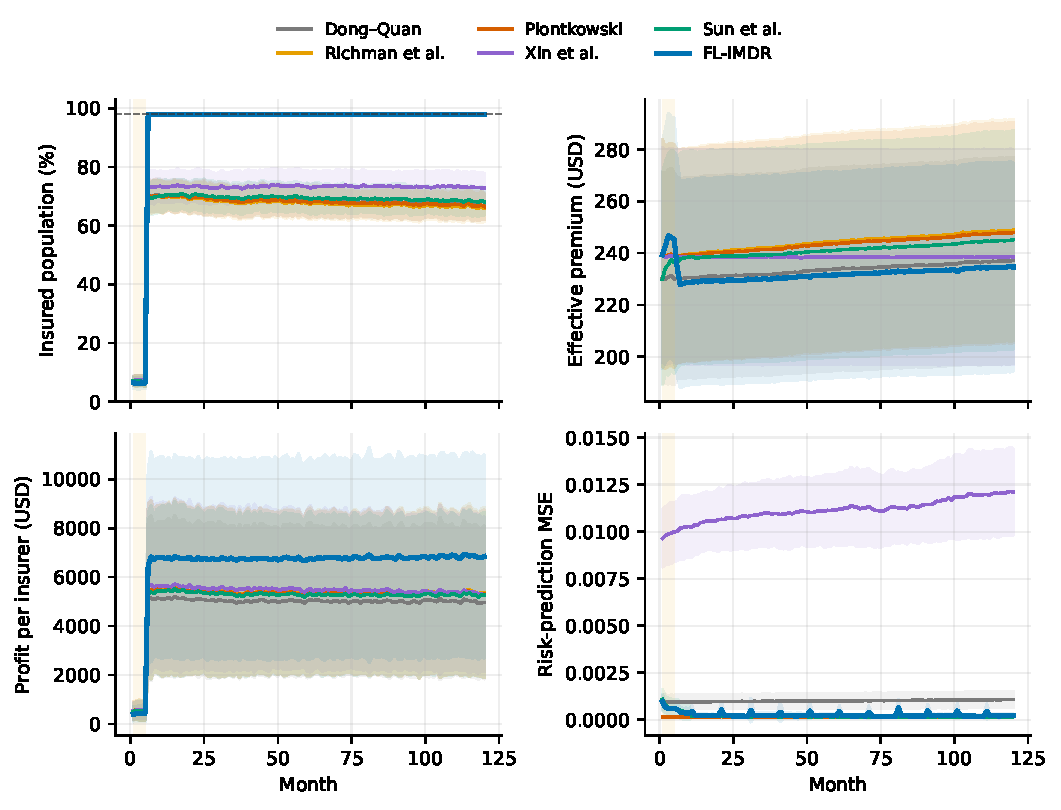
\includegraphics[width=0.94\textwidth]{figures/study_aligned_dynamics.pdf}
    \caption{Reference-calibrated common-environment trajectories over $50$
    paired seeds. Curves show the mean and shaded regions show $\pm$ one
    standard deviation. The shaded initial interval denotes the five-month
    lock-in period.}
    \label{fig:study_aligned_dynamics}
\end{figure*}

FL-IMDR reaches the locked $98\%$ enrollment target, compared with
$66.34\%$--$73.09\%$ for the cited study-aligned methods, corresponding to a
paired improvement of $24.91$--$31.66$ percentage points. Its accepted price
is $2.41$--$14.08 lower and its profit per insurer is
$1{,}461.85$--$1{,}848.63$ higher. All of these paired differences remain
significant after Holm correction
($p_{\mathrm{Holm}}\leq0.013$). The zero standard deviation of final-window
enrollment is structural because mandated enrollment enforces the specified
$98\%$ target in every final-window replication; it does not imply that the
other outcomes are deterministic.

\begin{table*}[t]
\centering
\caption{Predictive, plan-quality and competition outcomes in the same reference-calibrated experiment. Entries are mean $\pm$ standard deviation over 50 paired seeds.}
\label{tab:external_prediction_fairness}
\renewcommand{\arraystretch}{1.12}
\begin{adjustbox}{width=\textwidth}
\begin{tabular}{lcccc}
\toprule
Method & Accepted coverage (\%) & Risk MSE & Risk-group gap (pp) & HHI \\
\midrule
Dong--Quan AutoML-aligned~\cite{DongQuan2025} & 72.12 $\pm$ 1.87 & 0.001065 $\pm$ 0.000428 & 60.59 $\pm$ 9.47 & 0.639 $\pm$ 0.186 \\
Richman \emph{et al.} credibility-aligned~\cite{Richman2025} & 73.85 $\pm$ 0.55 & 0.000156 $\pm$ 0.000009 & 59.88 $\pm$ 9.19 & 0.726 $\pm$ 0.049 \\
Piontkowski small-portfolio-aligned~\cite{Piontkowski2025} & 74.98 $\pm$ 0.56 & 0.000156 $\pm$ 0.000009 & 59.07 $\pm$ 9.17 & 0.726 $\pm$ 0.049 \\
Xin \emph{et al.} fairness-aligned~\cite{Xin2025} & 69.58 $\pm$ 1.01 & 0.012046 $\pm$ 0.002256 & 33.89 $\pm$ 9.88 & 0.667 $\pm$ 0.159 \\
Sun \emph{et al.} FHE--CRL-aligned~\cite{Sun2026} & \textbf{76.40 $\pm$ 0.55} & \textbf{0.000156 $\pm$ 0.000009} & 57.55 $\pm$ 9.38 & 0.731 $\pm$ 0.048 \\
\textbf{FL-IMDR (proposed)} & 72.75 $\pm$ 0.76 & 0.000231 $\pm$ 0.000127 & \textbf{7.94 $\pm$ 0.30} & \textbf{0.458 $\pm$ 0.033} \\
\bottomrule
\end{tabular}
\end{adjustbox}
\end{table*}


The distributional improvement is also visible in the risk-group coverage
gap, which decreases to $7.94\pm0.30$ percentage points from
$33.89$--$60.59$ percentage points, while HHI falls to
$0.458\pm0.033$. Sun et al.'s study-aligned collective-learning comparator
obtains the highest accepted-plan coverage, while the Richman, Piontkowski and
Sun comparators attain nearly identical lowest risk MSE values. FL-IMDR therefore does not
achieve its market-level advantage through uniformly superior prediction.
Rather, target feedback, transfers and mandated enrollment change which
patients can enter the insured pool, while DP perturbation retains the
privacy--utility trade-off discussed in Section~\ref{app:dp_impact}.

\begin{table}[t]
\centering
\caption{Paired Wilcoxon tests comparing FL-IMDR with each study-aligned baseline. Holm correction is applied separately within each metric.}
\label{tab:external_significance}
\footnotesize
\begin{tabular}{llcc}
\toprule
Metric & Comparator & Paired $\Delta$ & $p_{\mathrm{Holm}}$ \\
\midrule
Insured population (pp) & Dong–Quan & 30.90 & $<0.001$ \\
Insured population (pp) & Richman et al. & 31.66 & $<0.001$ \\
Insured population (pp) & Piontkowski & 31.05 & $<0.001$ \\
Insured population (pp) & Xin et al. & 24.91 & $<0.001$ \\
Insured population (pp) & Sun et al. & 29.65 & $<0.001$ \\
Effective premium & Dong–Quan & -2.41 & 0.013 \\
Effective premium & Richman et al. & -14.08 & $<0.001$ \\
Effective premium & Piontkowski & -13.19 & $<0.001$ \\
Effective premium & Xin et al. & -4.01 & $<0.001$ \\
Effective premium & Sun et al. & -10.32 & $<0.001$ \\
Profit per insurer & Dong–Quan & 1848.63 & $<0.001$ \\
Profit per insurer & Richman et al. & 1461.85 & $<0.001$ \\
Profit per insurer & Piontkowski & 1499.82 & $<0.001$ \\
Profit per insurer & Xin et al. & 1480.11 & $<0.001$ \\
Profit per insurer & Sun et al. & 1573.46 & $<0.001$ \\
Risk-group coverage gap (pp) & Dong–Quan & -52.65 & $<0.001$ \\
Risk-group coverage gap (pp) & Richman et al. & -51.94 & $<0.001$ \\
Risk-group coverage gap (pp) & Piontkowski & -51.13 & $<0.001$ \\
Risk-group coverage gap (pp) & Xin et al. & -25.94 & $<0.001$ \\
Risk-group coverage gap (pp) & Sun et al. & -49.61 & $<0.001$ \\
\bottomrule
\end{tabular}
\end{table}


\begin{figure}[t]
    \centering
    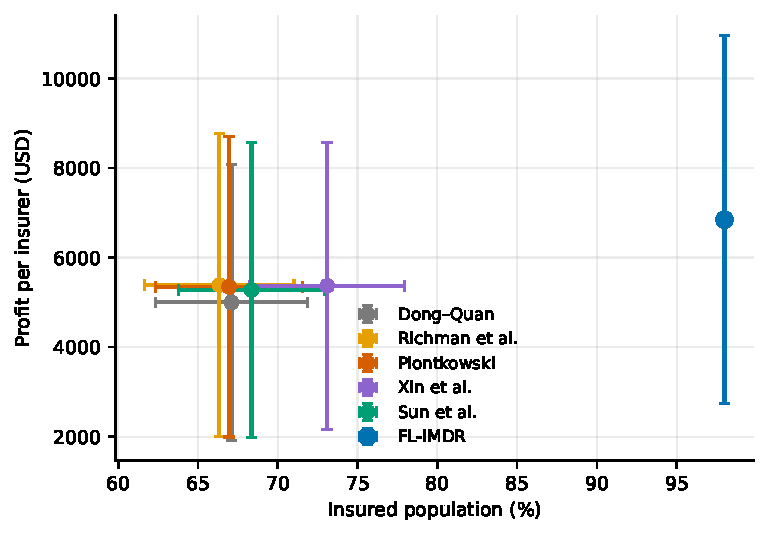
\includegraphics[width=\columnwidth]{figures/coverage_profit_frontier.pdf}
    \caption{Reference-calibrated steady-state insured-population--profit
    comparison. Markers show means; horizontal and vertical error bars show one
    standard deviation across paired seeds.}
    \label{fig:study_aligned_frontier}
\end{figure}

This is an internal synthetic comparison of market mechanisms. It does not
establish external actuarial calibration, real-market welfare effects, formal
privacy accounting for the selected noise scale, or cryptographic efficiency.
Exact reproduction of the cited studies would require their original data,
released implementations and application-specific evaluation targets.
